\underline{\textbf{Issue 1: For enumerate, the lines overflow too much horizontally}}

\begin{enumerate}
\item \textbf{Modulus Switch:} Switch the modulus of $\textsf{LWE}_{\vec{s}, \sigma}(\Delta m)$ From $q \rightarrow 2n$, which is from $64 \rightarrow 32$. After the modulus switch, the original LWE ciphertext is converted as follows:

$\mathbb{Z}_{2n=32} = \{-16, -15, -14, \gap{$\cdots$}, 13, 14, 15\}$

$\vec{s} = (1, 0, 0, 1, 1, 1, 0, 1) = \mathbb{Z}_2^{k=8}$


$\hat{\Delta} = \Delta\dfrac{2n}{64} = 8\dfrac{32}{64} = 4$

$\hat{\Delta}m = 4 \cdot 1 = 4 \in \mathbb{Z}_{2n=32}$

$\hat{e} =  \left\lceil e \dfrac{2n}{q} \right\rfloor = \left\lceil 2\dfrac{32}{64} \right\rfloor = 1 \in \mathbb{Z}_{2n=32}$

$ $

$\textsf{LWE}_{\vec{s}, \sigma}(\hat{\Delta}m) = (\hat{a}_0, \hat{a}_1, \hat{a}_2, \hat{a}_3, \hat{a}_4, \hat{a}_5, \hat{a}_6, \hat{a}_7, \hat{b}) \in \mathbb{Z}_{2n=32}^{k+1=9}$


$ = (\Big\lceil 8\dfrac{32}{64} \Big\rfloor, \Big\lceil -28\dfrac{32}{64}\Big\rfloor, \Big\lceil 4\dfrac{32}{64}\Big\rfloor, \Big\lceil -32\dfrac{32}{64}\Big\rfloor, \Big\lceil 0\dfrac{32}{64}\Big\rfloor, \Big\lceil 31\dfrac{32}{64}\Big\rfloor, \Big\lceil -6\dfrac{32}{64}\Big\rfloor, \Big\lceil 7\dfrac{32}{64}\Big\rfloor, \Big\lceil 24\dfrac{32}{64}\Big\rfloor)$

$ $

$= (4, {-14}, 2, -16, 0, 16, {-3}, 4, 12)$

$ $

Note that $\sum\limits_{i=0}^{7}(\hat{a}_is_i) + \hat{\Delta}m + \hat{e} = (4 - 16 + 16 + 4) + 4 + 1 = 13 \in \mathbb{Z}_{2n=32}$

$ $

$\hat b = 12 \approx 13 = \sum\limits_{i=0}^{7}(\hat{a}_is_i) + \hat{\Delta}m + \hat{e}$

This small difference in $\hat b$ comes from the aggregated noises of rounding $\hat a_0, \hat a_1, \cdots , \hat e$ during the modulus switch. 


\item \textbf{Blind Rotation:} We assume that the application avoids the problem of negacyclic polynomial rotation by ensuring that the usable plaintext values are the following continuous $\dfrac{8}{2}$ modulo values within $\mathbb{Z}_8 = \{-4, -3, -2, -1, 0, 1, 2, 3\}$, which are $\{-2, -1, 0, 1\}$. This implies that the only possible values of $i=\hat\Delta m + \hat e$ in $V(X)\cdot X^{i}$ will be: $i = \{-8, -7, \cdots, 6, 7\}$. Based on these requirements, \autoref{tab:lut} is the Lookup Table polynomial $V(X)$ that maps $\hat{\Delta} m + \hat{e}$ to $\Delta m$. 


\begin{table}[h]
\centering
\noindent\adjustbox{max width=\columnwidth}{
\begin{tabular}{|c||c|c|c|c|c|c|c|c|c|c|} % left align
\hline
% remove line in a table, \usepackage{adjustbox}
\multicolumn{10}{|l|}{$V(X) = v_0 + v_1X + v_2X^2 + v_3X^3 + v_4X^4 + v_5X^5 + v_6X^6 + v_7X^7$}  \\ 
\multicolumn{10}{|l|}{\textcolor{white}{......} $ + v_8X^8 + v_9X^9 + v_{10}X^{10} + v_{11}X^{11} + v_{12}X^{12} + v_{13}X^{13} + v_{14}X^{14} + v_{15}X^{15}$}  \\ 
\multicolumn{10}{|l|}{\textcolor{white}{....}$= 0 + 0X +0X^2 +0X^3 +1X^4 +1X^5 +1X^6 +1X^7$}  \\ 
\multicolumn{10}{|l|}{\textcolor{white}{......}$+ 2X^8  + 2X^9 + 2X^{10} + 2X^{11} + 1X^{12} + 1X^{13} + 1X^{14} + 1X^{15}$} \\ 
\hline
\hline
\textbf{\boldmath$i = \hat{\Delta}m + \hat{e}$} & $-8$ & $-7$ & $-6$ & $-5$ & $-4$ & $-3$ & $-2$ & $-1$ \\
(in $V \cdot X^{-i}$) & ($\textcolor{cyan}{}\textcolor{orange}{110}\textcolor{green}{00}_2$) & ($\textcolor{cyan}{}\textcolor{orange}{110}\textcolor{green}{01}_2$) & ($\textcolor{cyan}{}\textcolor{orange}{110}\textcolor{green}{10}_2$) & ($\textcolor{cyan}{}\textcolor{orange}{110}\textcolor{green}{11}_2$) & ($\textcolor{cyan}{}\textcolor{orange}{111}\textcolor{green}{00}_2$) & ($\textcolor{cyan}{}\textcolor{orange}{111}\textcolor{green}{01}_2$) & ($\textcolor{cyan}{}\textcolor{orange}{111}\textcolor{green}{10}_2$) & ($\textcolor{cyan}{}\textcolor{orange}{111}\textcolor{green}{11}_2$)\\
\hline
\textbf{constant term's} & $-2$ & $-2$ & $-2$ & $-2$ & $-1$ & $-1$ & $-1$ & $-1$ \\
 \textbf{coeff. of $V\cdot X^{-i}$}& $\textcolor{orange}{110}_2$ & $\textcolor{orange}{110}_2$ & $\textcolor{orange}{110}_2$ & $\textcolor{orange}{110}_2$ & $\textcolor{orange}{111}_2$ & $\textcolor{orange}{111}_2$ & $\textcolor{orange}{111}_2$ & $\textcolor{orange}{111}\textcolor{green}{00}_2$ \\
\hline
\textbf{$\bm{m}$ (plaintext)} & $-2$ & $-2$ & $-2$ & $-2$ & $-1$ & $-1$ & $-1$ & $-1$ \\
\hline
\hline
\textbf{\boldmath$i = \hat{\Delta}m + \hat{e}$} & $0$ & $1$ & $2$ & $3$ & $4$ & $5$ & $6$ & $7$ \\
(in $V \cdot X^{-i}$) & ($\textcolor{cyan}{}\textcolor{orange}{000}_2$)& ($\textcolor{cyan}{}\textcolor{orange}{000}_2$)& ($\textcolor{cyan}{}\textcolor{orange}{000}_2$)& ($\textcolor{cyan}{}\textcolor{orange}{000}_2$)& ($\textcolor{cyan}{}\textcolor{orange}{001}_2$)& ($\textcolor{cyan}{}\textcolor{orange}{001}_2$)& ($\textcolor{cyan}{}\textcolor{orange}{001}_2$)&($\textcolor{cyan}{}\textcolor{orange}{001}_2$)\\
\hline
\textbf{constant term's} & $0$ & $0$ & $0$ & $0$ & $1$ & $1$ & $1$ & $1$ \\
\textbf{coeff. of $V\cdot X^{-i}$}& $\textcolor{orange}{000}\textcolor{green}{00}_2$ & $\textcolor{orange}{000}\textcolor{green}{00}_2$ & $\textcolor{orange}{000}\textcolor{green}{00}_2$ & $\textcolor{orange}{000}\textcolor{green}{00}_2$ & $\textcolor{orange}{001}\textcolor{green}{00}_2$ & $\textcolor{orange}{001}\textcolor{green}{00}_2$ & $\textcolor{orange}{001}\textcolor{green}{00}_2$ & $\textcolor{orange}{001}\textcolor{green}{00}_2$ \\
\hline
\textbf{$\bm{m}$ (plaintext)} & $0$ & $0$ & $0$ & $0$ & $1$ & $1$ & $1$ & $1$ \\
\hline
\end{tabular}}
\centering
\caption{The Lookup Table for $n=16, q=64, t=8$ LWE setup.
\textcolor{orange}{Orange} is the plaintext $m$'s bits. \textcolor{green}{Green} is the noise $e$'s bits. %\textcolor{cyan}{Cyan} is the 0-padding bit at the MSB of $\hat\Delta m + e$ (and thus the MSB of $m$), ensured by the application's usage of plaintext numbers.
}
\label{tab:lut}
\end{table}

Note that $V(X)$'s coefficients for the $X^8 \sim X^{15}$ terms are $\{2, 1\}$ instead of $\{-2, -1\}$, so that if $V$ gets rotated by $\{-8,-7,-6,-5,4,5,6,7\}$ slots to the left, the constant term's coefficient flips its sign to $\{-2, -1\}$ due to wrapping around the boundary of the $n$ exponent. 

During the actual bootstrapping, we will do blind rotation of \autoref{tab:lut}'s $V(X)$ (which is GLWE-encrypted) by $\hat{b} - \sum\limits_{i=0}^{7}\hat{a}_is_i = 4$ positions to the left, which computed as follows:

$\hat\Delta m + \hat e = \hat{b} - \sum\limits_{i=0}^{7}\hat{a}_is_i = 12 - (4 - 16 + 16 + 4) = 4 \text{ mod 32} \in \mathbb{Z}_{2n=32}$ 


In \autoref{tab:lut}, if the rotation count $i = 4$, the corresponding constant term coefficient is $v_4 = 1 = m$. As $\Delta = 4$, we finally get $\textsf{LWE}_{\vec{s},\sigma}(\Delta m) = 1$. 



$ $

The actual blind rotation is computed as follows:

$\vec{s} = (1, 0, 0, 1, 1, 1, 0, 1)$

$\textsf{LWE}_{\vec{s}, \sigma}(\hat{\Delta}m) = (\hat{a}_0, \hat{a}_1, \hat{a}_2, \hat{a}_3, \hat{a}_4, \hat{a}_5, \hat{a}_6, \hat{a}_7, \hat{b}) =  (4, -14, 2, -16, 0, 16, -3, 4, 12)$

$V_0 = V \cdot X^{-\hat{b}} = V \cdot X^{-12} = v_{12} + v_{13}X + v_{14}X^2 + \cdots $

$V_1 = V_0 \cdot X^{\hat{a}_0s_0} = s_0 \cdot (V_0 \cdot X^{a_0} - V_0) + V_0 = V_0 \cdot X^{4} = v_{8} + v_{9}X + v_{10}X^2 + \cdots$ 

$V_2 = V_1 \cdot X^{\hat{a}_1s_1} = s_1 \cdot (V_1 \cdot X^{a_1} - V_1) + V_1 = V_1 = v_{8} + v_{9}X + v_{10}X^2 + \cdots$

$V_3 = V_2 \cdot X^{\hat{a}_2s_2} = s_2 \cdot (V_2 \cdot X^{a_2} - V_2) + V_2 = V_2 = v_{8} + v_{9}X + v_{10}X^2 + \cdots$

$V_4 = V_3 \cdot X^{\hat{a}_3s_3} = s_3 \cdot (V_3 \cdot X^{a_3} - V_3) + V_3 = V_3 \cdot X^{-16} = -v_{8} - v_{9}X - v_{10}X^2 - \cdots$

$V_5 = V_4 \cdot X^{\hat{a}_4s_4} = s_4 \cdot (V_4 \cdot X^{a_4} - V_4) + V_4 = V_4 \cdot X^{0} = -v_{8} - v_{9}X - v_{10}X^2 - \cdots$

$V_6 = V_5 \cdot X^{\hat{a}_5s_5} = s_5 \cdot (V_5 \cdot X^{a_5} - V_5) + V_5 = V_5 \cdot X^{16} = v_{8} + v_{9}X + v_{10}X^2 + \cdots$

$V_7 = V_6 \cdot X^{\hat{a}_6s_6} = s_6 \cdot (V_6 \cdot X^{a_6} - V_6) + V_6 = V_6 = v_{8} + v_{9}X + v_{10}X^2 + \cdots$

$V_8 = V_7 \cdot X^{\hat{a}_7s_7} = s_7 \cdot (V_7 \cdot X^{a_7} - V_7) + V_7 = V_7 \cdot X^{4} = v_{4} + v_5X + v_6X^2 + \cdots $

$ $

The final output of blind rotation is the GLWE ciphertext of $V_8$, $\textsf{GLWE}_{\vec{S}, \sigma}(V_8)$, whose constant term's coefficient is $v_4 = m = 1$. 

$ $

Each step of the actual blind rotation above is computed as the following TFHE ciphertext-to-ciphertext multiplication:

$\textsf{GLWE}_{\vec{S}, \sigma}(V_{i+1}) = \textsf{GGSW}_{\vec{S}, \sigma}^{\beta, l}(s_i) \cdot (\textsf{GLWE}_{\vec{S}, \sigma}(V_i) \cdot X^{a_0} - \textsf{GLWE}_{\vec{S}, \sigma}(V_i)) + \textsf{GLWE}_{\vec{S}, \sigma}(V_i)$

$ $

We will leave this computation for the reader's exercise.

$ $

\item \textbf{Coefficient Extraction:} At the end of blind rotation, we finally get the following GLWE ciphertext:

$\textsf{GLWE}_{\vec{S}, \sigma}(V_8)$

$ = \textsf{GLWE}_{\vec{S}, \sigma}\bm(\Delta \cdot (v_4 + v_5X + v_6X^2 + v_7X^3 + v_8X^{4} + v_9X^{5} + v_{10}X^{6} + v_{11}X^{7} + v_{12}X^{8} + v_{13}X^{9} + v_{14}X^{10} + v_{15}X^{11} - v_{0}X^{12} - v_{1}X^{13} - v_{2}X^{14} - v_{3}X^{15})\bm)$

$ = \textsf{GLWE}_{\vec{S}, \sigma}\bm(\Delta\cdot(1 + 1X + 1X^2 + 1X^3 + 2X^{4} + 2X^{5} + 2X^{6} + 2X^{7} + 1X^{8} + 1X^{9} + 1X^{10} + 1X^{11} - 0X^{12} - 0X^{13} - 0X^{14} - 0X^{15})\bm)$

$ = \left(A_0 = \sum\limits_{j=0}^{15}(a_{0,0} + a_{0,1}X + \cdots), A_1 = \cdots, A_{k-1} = \cdots, B = \sum\limits_{j=0}^{15}b_{j}X^j\right)$

Now, we extract the constant term's coefficient of the encrypted polynomial $\textsf{GLWE}_{\vec{S}, \sigma}(\Delta \cdot (1 + 1X + 1X^2 + \cdots))$ by using the coefficient extraction formula (Summary~\ref{subsec:tfhe-extraction}). Specifically, we will extract the constant term's coefficient, which corresponds to $\textsf{LWE}_{\vec{s}, \sigma}(\Delta m_0)$. We extract $\textsf{LWE}_{\vec{s}, \sigma}(\Delta m_0)$ by computing the following:

$\textsf{LWE}_{\vec{s}, \sigma}(\Delta m_0) = (a_0', a_1', \gap{$\cdots$} , a_k', b_h)$

\[
    \text{, where } a'_{n \cdot i + j} =   
\begin{cases}
    a_{i,0 - j} \text{ (if } 0 \leq j \leq 0\text{)}\\
    a_{i,n + 0 - j} \text{ (if } 0+1 \leq j \leq n-1\text{)}\\
\end{cases}
, b_0 \text{ is obtained from the polynomial } B
\]


\end{enumerate}






$ $

\subsubsection{Discussion}
\label{subsubsec:polynomial-ring-discuss}


\underline{\textbf{Issue 2: The table's upper margin is truncated}}

\begin{table}[h]
\centering
\noindent\adjustbox{max width=\columnwidth}{
\begin{tabular}{|c||c|c|} % left align
\hline
&\textbf{Integer Ring} & \textbf {Polynomial Ring} \\
\hline
\hline
\textbf{{Set Elements}} & number & polynomial \\
\hline
\textbf{{Ring Notation}} & $\mathbb{Z}_p = \{0, 1, \gap{$\cdots$}, p - 1\}$  & $\mathbb{Z}_p[x] / (x^n + 1)$ \\
\textbf{{\& Definition}} & A set of all integers between $0$ and $p$ & A set of all polynomials $f$ such that\\
&& $f= c_0 + c_1x^1 + c_2x^2 \cdots + c_{n-1}x^{n-1}$ \\
&& where each coefficient $c_i \in \mathbb{Z}_p$ \\
&& and $f$'s degree is less than $n$ \\
\hline
\textbf{{Supported}}&$(+, \cdot)$& $(+, \cdot)$ \\
\textbf{{Operations}}&(Addition, Multiplication)& (Addition, Multiplication) \\
\hline
\textbf{{($+$) Operation}} & We know how to add numbers & $f_a = a_0 + a_1x^1 + a_2x^2 \cdots + a_{d_a-1}x^{d_a-1}$ \\
 & & $f_b = b_0 + b_1x^1 + b_2x^2 \cdots + b_{d_b-1}x^{d_b-1}$ \\
 & & Then, $f_a + f_b$ is computed as: \\
 & & $f_c = \sum\limits_{i=0}^{\textsf{max}(d_a,d_b)}(a_i+b_i)x^i$ \\
\hline
\textbf{{($\cdot$) Operation}} & We know how to multiply numbers & $f_a = a_0 + a_1x^1 + a_2x^2 \cdots + a_{d_a-1}x^{d_a-1}$ \\
 & & $f_b = b_0 + b_1x^1 + b_2x^2 \cdots + b_{d_b-1}x^{d_b-1}$ \\
 & & Then, $f_a \cdot f_b$ is computed as: \\
 & & $f_c = \sum\limits_{i=0}^{d_a+d_b}\sum\limits_{j=0}^{i}a_jb_{i-j}x^i$ \\
\hline
& For $a, b \in \mathbb{Z}_p$ & For $f_a, f_b \in \mathbb{Z}_p[X]/(x^x + 1)$,\\
\textbf{{Commutative}}  & $ a + b = b + a$ & $f_a + f_b = f_b + f_a$\\
\textbf{{Associative}} & $(a + b) + c = a + (b + c)$ & $(f_a + f_b) + f_c = f_a + (f_b + f_c)$\\
\textbf{{Distributive}} & $a \cdot (b + c) = a\cdot b + a\cdot c$ & $f_a \cdot (f_b + f_c) = f_a\cdot f_b + f_a\cdot f_c$\\
\textbf{{Closed}}& $a + b \equiv c \in \mathbb{Z}_p$, $a \cdot b \equiv d \in \mathbb{Z}_p$ & $f_a + f_b \equiv f_c \in \mathcal{R}_{\langle n, q \rangle}$, \\
&&$f_a \cdot f_b \equiv f_d \in \mathcal{R}_{\langle n, q \rangle}$\\
\hline
\textbf{{Congruency ($\equiv$)}} & Two numbers $a \equiv b$ in modulo $p$ if: & Two polynomials $f_a \equiv f_b$ in $\mathbb{Z}_p[x] / (x^n + 1)$ if:    \\
 & $(a \gap{\text{mod}} p) = (b \gap{\text{mod}} p)$   & $f'_a = f_a \gap{\text{mod}} (x^n + 1) = \sum\limits_{i=0}^{d_a} a_ix^i$ \\
 & & $f'_b = f_b \gap{\text{mod}} (x^n + 1) = \sum\limits_{i=0}^{d_b} b_ix^i$, \\
&& $d_a = d_b$ and $a_i \equiv b_i$ in modulo $p$\\
&&for all $0 \leq i \leq d_a$\\ 
\hline
\end{tabular}}
\centering
\caption{Comparison between a number ring and a polynomial ring.
}
\label{tab:ring-comparison}
\end{table}


\underline{\textbf{Issue 3: Math error in a table}}

\begin{table}[h] %usepackage{array} 
\begin{tabular}{|>{\centering\arraybackslash}p{0.1\columnwidth}||>{\centering\arraybackslash}p{0.4\columnwidth}||>{\centering\arraybackslash}p{0.4\columnwidth}|}
\hline \hline
& \textbf{Polynomial over $\bm{X} \bm{\in} \bm{\mathbb{C}}$} & \textbf{Polynomial over $\bm{X} \in \bm{\mathbb{Z}}_{\bm{p}}$} \\ 
& \textbf{(Complex Number)} & \textbf{(Integer Ring)} \\ \hline \hline
\textbf{Definition of the $\bm \mu$-th Root of Unity}& All $X \in \mathbb{C}$ such that $X^\mu = 1$, (which are computed as $X = e^{2 \pi i k / \mu}$ for integer $k$ where $0 \leq k \leq \mu - 1$)& All $X \in \mathbb{Z}_p$ such that $X^\mu \equiv 1 \bmod p$\\ \hline
\textbf{Definition of the Primitive $\bm \mu$-th Root of Unity}& Those $\mu$-th roots of unity $\omega$ such that $\omega^{\mu} = 1$, and $\omega^{\frac{\mu}{2}} \neq 1$ &  Those $\mu$-th roots of unity $\omega$ such that $\omega^{\mu} \equiv 1 \bmod p$, and $\omega^{\frac{\mu}{2}} \not\equiv 1 \bmod p$ \\ \hline
\textbf{Definition of the $\bm \mu$-th Cyclotomic Polynomial} & \multicolumn{2}{|c|}{\shortstack{The polynomial whose roots are the $\mu$-th primitive roots of unity as follows: \\ $ \Phi_{\mu}(x) = \prod_{\omega \in P(\mu)} (x - \omega) $  \text{ } (see Definition~\ref*{subsec:cyclotomic-def} in \autoref{subsec:cyclotomic-def})}}\\ \hline
\textbf{Finding Primitive $\bm \mu$-th Roots of Unity} & For $\omega = e^{2 \pi i/ \mu}$, compute all $\omega^k$ such that $0 < k < \mu $ and $\textsf{gcd}(k, \mu) = 1$  (Theorem~\ref*{subsec:roots-theorem}.4 in \autoref{subsec:roots-theorem}) & Find one satisfactory $\omega$ that is a root of the $\mu$-th cyclotomic polynomial, and compute all $\omega^k \bmod p$ such that $0 < k < \mu $ and $\textsf{gcd}(k, \mu) = 1$ \\ \hline \hline
\end{tabular}
\caption{The roots of unity and cyclotomic polynomials over $X \in \mathbb{C}$ v.s. over $X \in \mathbb{Z}_p$}
\label{tab:cyclotomic-polynomial-comparison}
\end{table}

$ $

\underline{\textbf{Issue 4: Math error (how can I modify the below to make it appear without any error?}}

$\mathcolor{white}{A(X)} = \underbrace{\underbrace{(\underbrace{A_{0,0}(X^4)}_{\text{\textcolor{red}{FFT Level 1}}} + X^2\cdot \underbrace{A_{0,1}(X^4)}_{\text{\textcolor{red}{FFT Level 1}}})}_{\text{\textcolor{red}{FFT Level 2}}} + X \cdot \underbrace{(\underbrace{A_{1,0}(X^4)}_{\text{\textcolor{red}{FFT Level 1}}} + X^2\cdot \underbrace{A_{1,1}(X^4)}_{\text{\textcolor{red}{FFT Level 1}}})}_{\text{\textcolor{red}{FFT Level 2}}}}_{\text{\textcolor{red}{FFT Level 3}}}$



$ $

\underline{\textbf{Issue 5: Line Overflow}}

\begin{tcolorbox}[title={\textbf{\tboxlabel{\ref*{subsec:glwe-alternative}} An Alternative GLWE Cryptosystem}}]

\textbf{\underline{Initial Setup}:} $\Delta = \left\lfloor\dfrac{q}{t}\right\rfloor$, $\{S_i\}_{i=0}^{k-1} \xleftarrow{\$} \mathcal{R}_{\langle n, 2 \rangle}^k$

$ $

\par\noindent\rule{\textwidth}{0.4pt}


\textbf{\underline{Encryption Input}:} $M \in \mathcal{R}_{\langle n, t \rangle}$, $\{A_i\}_{i=0}^{k-1} \xleftarrow{\$} \mathcal{R}_{\langle n,q \rangle}^{k}$, $E \xleftarrow{\chi_\sigma} \mathcal{R}_{\langle n,q \rangle}$

$ $

\begin{enumerate}
\item Scale up $M \longrightarrow \Delta M \text { } \in \mathcal{R}_{\langle n, q\rangle}$

\item Compute $B = \textcolor{red}{-\sum\limits_{i=0}^{k-1}{(A_i \cdot S_i)}} + \Delta  M + E \text{ } \in \mathcal{R}_{\langle n,q \rangle}$

\item $\textsf{GLWE}_{S,\sigma}(\Delta M) = (\{A_i\}_{i=0}^{k-1}, B) \text{ } \in \mathcal{R}_{\langle n,q \rangle}^{k + 1}$ 

\end{enumerate}

\par\noindent\rule{\textwidth}{0.4pt}


\textbf{\underline{Decryption Input}:} $C = (\{A_i\}_{i=0}^{k-1}, B) \text{ } \in \mathcal{R}_{\langle n,q \rangle}^{k + 1}$

\begin{enumerate}
\item $\textsf{GLWE}^{-1}_{S,\sigma}(C) = B \text{ } \textcolor{red}{ + \sum\limits_{i=0}^{k-1}{(A_i \cdot S_i)}} = \Delta  M + E \text{ } \in \mathcal{R}_{\langle n,q \rangle}$

\item Scale down 
$\Bigl\lceil \dfrac{ \Delta  M + E }{\Delta}\Bigr\rfloor = M  \text{ } \in \mathcal{R}_{\langle n, t \rangle}$

\end{enumerate}

For correct decryption, every noise coefficient $e_i$ of polynomial $E$ should be: $e_i < \dfrac{\Delta}{2}$.

\end{tcolorbox}

$ $

\underline{\textbf{Issue 6: sin crashes when used in a caption (see the LaTeX source code that I commented out just below this)}}

%\begin{figure}[h!]
%    \centering
%  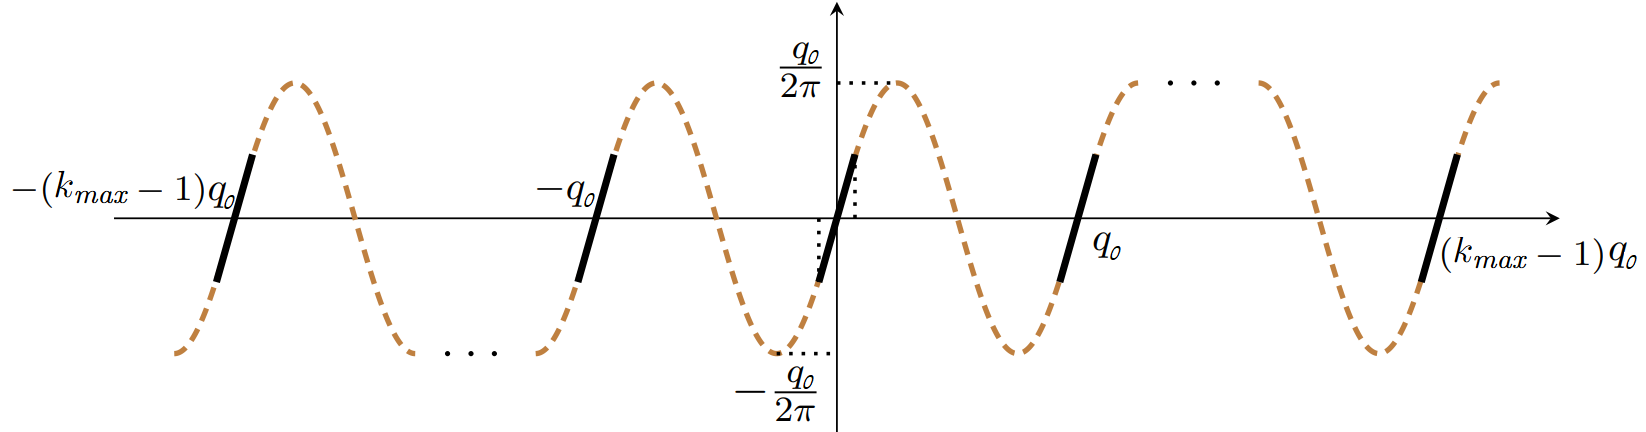
\includegraphics[width=1.0\linewidth]{figures/modulo-reduction-sine.png}
%  \caption{Sine function $f(x) = \dfrac{q_0}{2\pi}\cdot \sin \left(\dfrac{2\pi x}{q_0}\right)$ such that $f(\Delta m_i + e_i + q_0k_i) \approx \Delta m_i + e_i$ (provided $\Delta m_i + e_i \ll q_0$)}
%  \label{fig:modulo-reduction-sine}
%\end{figure}

$ $

\underline{\textbf{Issue 7: Matrix cuts vertically when seeing $\cdots$ twice}}

\noindent $\hathat{W}^* = \begin{bmatrix}
1 & (\omega^{J(0)}) & (\omega^{J(0)})^2 & \cdots & (\omega^{J(0)})^{n-1}\\
1 & (\omega^{J(1)}) & (\omega^{J(1)})^2 & \cdots & (\omega^{J(1)})^{n-1}\\
1 & (\omega^{J(2)}) & (\omega^{J(2)})^2 & \cdots & (\omega^{J(2)})^{n-1}\\
\vdots & \vdots & \vdots & \ddots & \vdots \\
1 & (\omega^{J(\frac{n}{2}-1)}) & (\omega^{J(\frac{n}{2}-1)})^2 & \cdots & (\omega^{J(\frac{n}{2}-1)})^{n-1}\\
1 & (\omega^{J_*(0)}) & (\omega^{J_*(0)})^2 & \cdots & (\omega^{J_*(0)})^{n-1}\\
1 & (\omega^{J_*(1)}) & (\omega^{J_*(1)})^2 & \cdots & (\omega^{J_*(1)})^{n-1}\\
1 & (\omega^{J_*(2)}) & (\omega^{J_*(2)})^2 & \cdots & (\omega^{J_*(2)})^{n-1}\\
\vdots & \vdots & \vdots & \ddots & \vdots \\
1 & (\omega^{J_*(\frac{n}{2}-1)}) & (\omega^{J_*(\frac{n}{2}-1)})^2 & \cdots & (\omega^{J_*(\frac{n}{2}-1)})^{n-1}\\
\end{bmatrix}$

$ $

\underline{\textbf{Issue 8: Using a special character in the math mode based on text}}
$\text{\rotatecharone{E}}^{T}$

$ $

\underline{\textbf{Issue 9: $\bmod$ error}}

\textcolor{red}{ \# where $y_i = \dfrac{q}{q_i} \text{, } z_i = y_i^{-1} \bmod q_i$, and $b = \prod\limits_{i=1}^lb_i$}

$ $

\underline{\textbf{Issue 10: A math input error}}
$\textsf{DecompMult\textsubscript{RNS}}(D_2, S^2_{\langle S, \textsf{RNS}\rangle}) = \textsf{RLWE}_{S, \sigma}(D_2 \cdot S^2) $

$ $

\underline{\textbf{Issue 11: Too small vertical gap between each section page's sub-section table and footnote hyperlinks}}

There is an enough space for each part page's table, but there isn't for each section page's table. Could you please add a single space between them? Also, could it be possible to add a title "Section Table" at the top of each section table in a section page?